%%%%%%%%%%%%%%%%%%%%% chapter.tex %%%%%%%%%%%%%%%%%%%%%%%%%%%%%%%%%
%
% sample chapter
%
% Use this file as a template for your own input.
%
%%%%%%%%%%%%%%%%%%%%%%%% Springer-Verlag %%%%%%%%%%%%%%%%%%%%%%%%%%
%\motto{Use the template \emph{chapter.tex} to style the various elements of your chapter content.}
\chapter{声纹识别}
\label{voiceprint} 

本章简单介绍声纹识别的概念,并其常见的算法,以及在实际中的应用。


\section{问题定义}

\subsection{基本定义}

声纹识别(Voice Print Recognition),也称作说话人识别(Speaker Recognition),是一种生物识别技术,能够根据说话人的声音特征提供精准、高效、便捷的身份识别服务。从感官直觉上来说,声纹虽然不像人脸、指纹的个体差异那样直观可见,但由于人在讲话时使用的发声器官--舌、牙齿、喉头、肺、鼻腔在尺寸和形态方面每个人的差异很大,因此反映到任何两个人的声纹图谱都存在有差异。最直观的感受是当我们打电话给认识的人的时候,通过很短一句话甚至一声“喂?”,就能准确地分辨出接电话的是谁。这种语音中承载的说话人身份信息的唯一性使得声纹也可以像人脸、指纹那样作为生物信息识别技术的生力军,可广泛应用于金融安全,公共安防,智能家居等领域。


\subsection{分类}

声纹识别通常分为两大类,说话人确认和说话人辨别,也就是常说的声纹1:1识别和声纹1:N识别。声纹1:1识别是指确认某段语音是否是指定的某个人所说的,而声纹1:N识别是判断某段语音是若干人中的哪一个所说的。不同的任务和应用会使用不同的声纹识别技术,如诈骗电话需要缩小人员范围时可能需要声纹1:N技术进行辨别,而银行金融交易时则需要声纹1:1识别技术进行确认。

从另一方面,声纹识别也分为文本相关(Text-Dependent)和文本无关(Text-Independent)两类。与文本相关的声纹识别要求用户按规定内容进行朗读,这样能更加准确的建立模型,在识别的时候也要求用户按规定内容朗读。文本无关的声纹识别并不要求用户根据指定文本进行朗读,这样也能建立模型,验证的时候同样不需要用户根据指定文本进行朗读。一般来说,文本相关的声纹识别效果会更好,安全性更高,但是用户体验较差和使用场景就相对较窄,通常用于安全要求比较高的场景,如金融核实身份。文本无关的声纹识别会和文本依赖比较弱,因此能进行跨语种使用,就算我们没有别的语种的语料,也是能应用到那语种上面去。文本无关的使用场景很宽广,在金融客服上就能建立声纹库,后面的用户在金融上快速验证和关联。

\subsection{挑战和机遇}

声纹识别技术的应用会有很多挑战,比如同一个人的声音具有易变性,可以控制不同部分造成不同发音;同时会受到身体状况、年龄、情绪等的影响,对识别性能有影响;又比如不同的麦克风、信道、环境噪音等对识别性能有比较大的干扰;又比如混合说话人的情形下人的声纹通常不易分离和识别等等。当然这些挑战也会被利用转化为优势,比如声音会受身体状况,年龄,情绪的影响,因此会单独训练出利用声纹识别情绪,或者利用声纹识别是否生病目前有应用到养猪场识别病猪等等。

尽管如此,与其他生物特征相比,声纹识别的应用有一些特殊的优势:
\begin{itemize}
	\item 获取声纹数据成本较低
	\item 用户使用接受程度较高
	\item 使用成本较低,适合远程身份确认
	\item 随着文本无关技术提升,能在小语种、跨种族等方向都有应用场景
\end{itemize}
这些优势受到系统开发者和用户青睐,从而使得声纹识别的应用越来越受到欢迎。

\section{实现方案}
声纹识别中通常的流程如图~\ref{pic:vpr}所示。不管是1:1还是1:N大致都是分为三部分:前置处理,特征抽取和声纹匹配。前置处理通常是VAD检测、反欺诈活体检测、声音增强等。VAD检测处理是把有声音部分和静音部分区分出来,把有声音部分送到后续处理中去。反欺诈活体检测是主要应对声纹识别是否被攻击,提高安全性。这些前置处理不在这里详细展开细说,匹配算法我们可以用最普通的计算向量距离如欧式距离或cos值,也可以用深度学习网络进行计算相似度。接下来我们重点介绍声纹的特征抽取。
\begin{figure*}
	\centering
	\subfigure[声纹1:1识别]
	{
		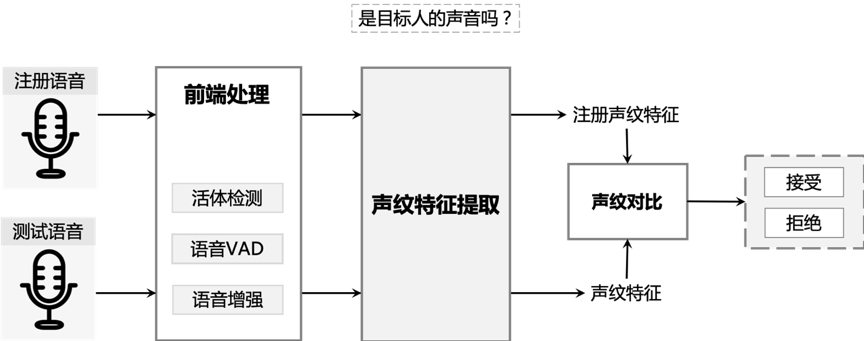
\includegraphics[width=0.46\textwidth]{img/chapter_voiceprint/vpr_1v1.png}
		\label{pic:vpr1v1}
	}
	\subfigure[声纹1:N识别]
	{
		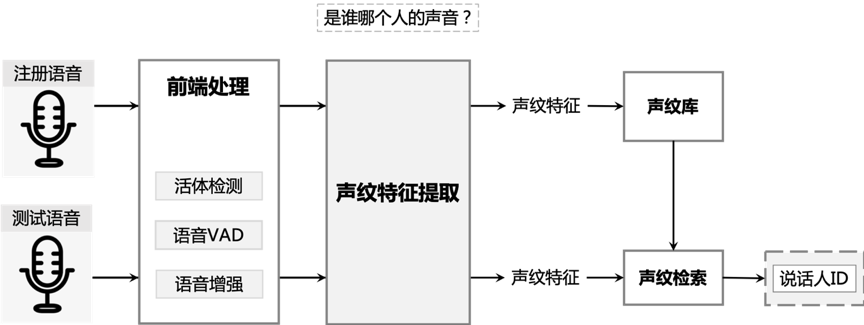
\includegraphics[width=0.46\textwidth]{img/chapter_voiceprint/vpr_1vn.png}
		\label{pic:vpr1vn}
	}
	\caption{声纹识别流程}
	\label{pic:vpr}
\end{figure*}

\subsection{特征抽取}
声纹识别的特征抽取大致经历了三代算法,GMM模型到ivector最后到深度学习网络。我们重点介绍前面两代,深度学习网络的方法和人脸特征抽取方法类似,也是分为两大类:度量学习(Metric Learning)和基于 margin的分类方法(Margin Based Classification),将会在人脸识别中重点介绍。

\subsubsection{GMM-UBM模型}
GMM模型~\cite{reynolds1995speaker}即高斯混合模型,是由多个高斯函数进行加权求和进行拟合复杂的函数,如
\begin{equation}
\label{eq:gmm}
\begin{aligned}
p(x) = \sum_{k=1}^K p(k)p(x|k) = \sum_{k=1}^K \pi_k N(x|\mu_k, \Sigma_k)
\end{aligned}
\end{equation}
其中,$\pi_k$表示第$k$个高斯函数的权重,$\mu_k$和$\Sigma_k$表示第$k$个高斯的均值和方差。

GMM模型的参数求解,一般使用EM算法进行求解。通常情况下,GMM模型可以平滑地逼近任意形状的函数,具备对实际数据极强的表征力。而声纹识别实际上就是从不同语音中抽取出相同的表征特征来。GMM模型同时还具备比较好的泛化能力。因此GMM模型在声纹识别初期获得比较好的效果。随着$k$的增大,所需要的训练数据也就更加大了,否则获取不到泛化能力较好的模型。

在实际使用过程中,每个人语音数据有限,很难获取到比较通用的声纹识别模型。为了解决这个问题,DA Reynolds提出了通用背景模型(Universal Background Model)~\cite{reynolds2000speaker},简称UBM。先使用大量和说话人无关的语音数据训练一个GMM模型,然后再使用少量的说话人数据,通过自适应算法(如最大后验概率MAP、最大似然线性回归MLLR等)获取到说话人的个性特征的模型叫做UBM模型。这个思想有点像现在深度学习的finetune思想。这个模型就是GMM-UBM模型。该模型参数可以减半并有更快收敛的特点。

随着实际应用,GMM-UBM的存在问题:参数仍然很大和受信道的干扰比较大。学术界提出了GMM-SVM模型~\cite{campbell2006svm}、JFA模型~\cite{kenny2005joint}等等去优化解决。

\subsubsection{ivector模型}
基于GMM-UBM的模型,基本是基于特征声纹空间与特征信道空间的独立假设,但是在现实使用中,数据之间都是具有相关性的。之前的假设更多是方便了公式推导同时也限制了模型的泛化能力。N.Dehak认为既然声纹信息与信道信息不能做到完全独立,那就用一个一段低维度的定长向量同时描述声纹信息和信道信息,从而提出了ivector模型~\cite{dehak2010front}。

对于每一段语音都有高斯均值向量$M$表示如下:
\begin{equation}
\label{eq:ivector}
\begin{aligned}
M = m + \omega T
\end{aligned}
\end{equation}
其中,$m$表示通用背景模型(UBM)的高斯均值向量,该值和声纹信息、信道信息无关,$\omega$是全局差异空间因子,即为ivector向量,它的先验服从标准正态分布$N(0,1)$,$T$表示全局的差异空间矩阵。接下来只需要估计$\omega$和$T$值即可。

对于$\omega$和$T$的参数估计,我们基于假设:每一段语音都来自不同的说话人。首先计算训练数据中每个说话人所对应的Baum-Welch统计量,随后随机产生T的初始值。后续采取EM算法估算得到相关的参数。


\section{应用案例}
\subsection{声纹1:1识别应用案例}
\subsubsection{电话客服核身}
在电话客服中应用声纹核身,可以节省核身时间,降低运营成本;并减少核身问题,提升客户体验;更重要的是,即使犯罪分子掌握了用户的所有信息,也能通过声音判断是否为本人,是否存在欺诈风险。例如,部分银行的服务热线目前已接入声纹核身技术,大致流程如图~\ref{pic:vprapp1}。

\begin{figure}[h!]
	\begin{center}
		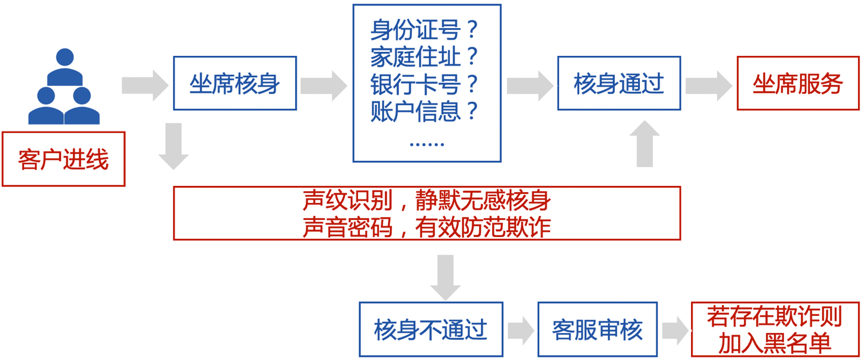
\includegraphics[width=0.8\textwidth]{img/chapter_voiceprint/vpr_app1.png}
		\caption{电话客服核身基本流程}
		\label{pic:vprapp1}
	\end{center}
\end{figure}

\subsubsection{社保核查}
声纹验证能够解决参保人员面临的远程和现场身份核查及生存验证的问题,避免了指纹验证和人脸识别等需要现场办理、不易采集、伪造等问题,有效杜绝冒领养老金的可能性,节约社保资金和人力成本。例如,印尼新一代养老金认证系统已通过声纹验证技术,使其250万离退休人员在领取养老金时可通过电话或手机app进行远程身份认证,不仅节省了大量人力投入,还显著降低了传统骗保率。

\subsubsection{声纹锁}
如图~\ref{pic:vprapp2}所示声纹验证可作为登录、密保、修改账户信息的一种验证方式,也可以应用于门禁/闸机等。

\begin{figure*}
	\centering
	\subfigure[声纹锁(一)]
	{
		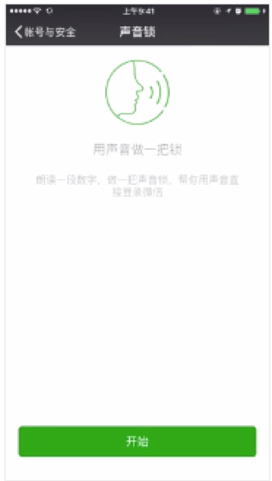
\includegraphics[width=0.3\textwidth]{img/chapter_voiceprint/vpr_app2a.png}
		\label{pic:vprapp2a}
	}
	\subfigure[声纹锁(二)]
	{
		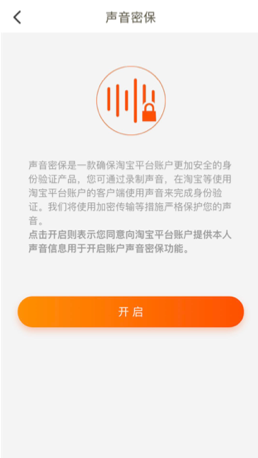
\includegraphics[width=0.3\textwidth]{img/chapter_voiceprint/vpr_app2b.png}
		\label{pic:vprapp2b}
	}
	\caption{声纹锁样例}
	\label{pic:vprapp2}
\end{figure*}

\subsubsection{声纹支付}

央行发布声纹识别安全应用技术标准,认定声纹技术可适用于手机银行、第三方支付,通过与语音交互硬件结合,能够解决无屏或远场进行身份验证的痛点。
\begin{figure*}
	\centering
	\subfigure[声纹支付]
	{
		
\includegraphics[width=0.6\textwidth]{img/chapter_voiceprint/vpr_app3a.png}
		\label{pic:vprapp3a}
	}
	\subfigure[声纹支付界面]
	{
		
\includegraphics[width=0.2\textwidth]{img/chapter_voiceprint/vpr_app3b.png}
		\label{pic:vprapp3b}
	}
	\caption{声纹支付样例}
	\label{pic:vprapp3}
\end{figure*}

\subsubsection{声纹唤醒}
通过声纹识别“主人”身份,只允许主人唤醒设备,或定制个性化服务,可适用于手机助手、智能音箱、智能家居、车载助手、服务机器人等智能设备。如图~\ref{pic:vprapp4}所示,在车联网应用中用户可以提前注册声纹信息并添加个性化配置,车机将通过声纹识别确认当前的驾驶人身份,可快速切换至对应的用户配置,令行车体验更加轻松。

\begin{figure}[h!]
	\begin{center}
		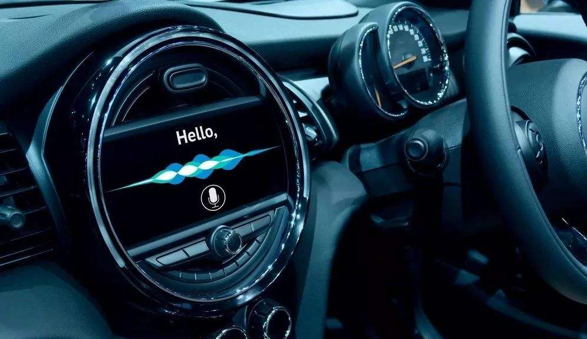
\includegraphics[width=0.6\textwidth]{img/chapter_voiceprint/vpr_app4.png}
		\caption{汽车声纹唤醒}
		\label{pic:vprapp4}
	\end{center}
\end{figure}


\subsection{声纹1:N识别应用案例}
\subsubsection{公安}
以破案、追逃为导向,利用声纹识别技术公安可进行“案查人”、“人查案”、“案查案”与“人查人”等多种排查方式:
\begin{itemize}
	\item 案查人:如电信诈骗,主要线索只有语音的情况下,将该语音进行声纹库大库检索,快速锁定嫌疑人。
	\item 人查案:公安抓捕到可疑人员后,提取出该人的声纹特征,将其放入尚未侦破的语音案件中,排查该人是否为在逃人员。
	\item 案查案:公安人员可使用声纹识别技术将尚未侦破的语音案件以及语音线索归纳整理,从中排查是否有多起案件是同一人所为,帮助侦察人员获得更多线索,提高排查效率。
	\item 人查人:公安机关在抓捕到可疑人员后,提取出该人的声纹特征,为避免该人使用伪造身份,可将其声纹特征放入已知人员的声纹库,查询其真实身份。
\end{itemize}

声纹识别技术还能应用于重点人员监管、反电信诈骗、反恐、刑事案件侦破、身份查询与核验,助力公安有效遏制与打击犯罪,构建和强化安全的社会公众环境。例如:
\begin{itemize}
	\item 反电信网络欺诈:在通信系统或安全监测系统中嵌入声纹识别技术,能够对黑名单人员语音对话实时预警,提示重点人员可疑行为;语音内容关键词识别动态预警,提示可疑案件与犯罪意图。
	\item 动态声纹布控:通过声纹识别和声纹大数据技术,进行对重点人员和关键卡口的布控监管,在第一时间完成举报人或嫌疑人身份鉴定,辅助刑事案件侦破和案情分析。
\end{itemize}

\begin{figure}[h!]
	\begin{center}
		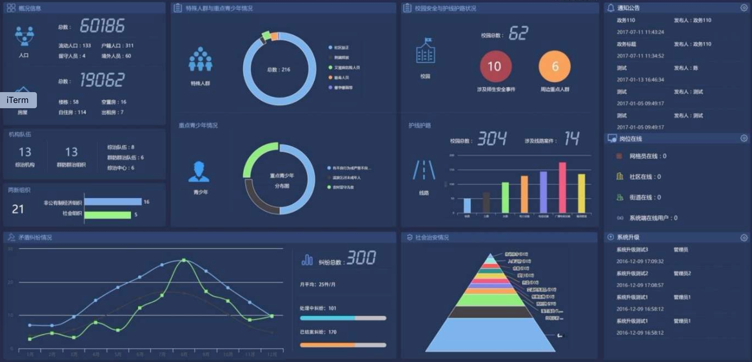
\includegraphics[width=0.8\textwidth]{img/chapter_voiceprint/vpr_app6.png}
		\caption{公安布控监管系统}
		\label{pic:vprapp6}
	\end{center}
\end{figure}

\subsubsection{金融黑名单识别}
将信贷黑名单、风险等级高、不良中介、金融欺诈等用户声纹加入黑名单库,当其再次办理业务时,匹配到黑名单库的用户,直接给出风险预警。例如,车险业务能够针对报假案、修理厂、黑中介等不良用户建立黑名单声纹库,当不良用户再次报案时,业务员端能够及时给出预警。

\subsubsection{客户定制化服务}
对于某些小群体用户,如银行VIP客户电话呼入时,可通过声纹1:N匹配VIP声纹库,识别用户身份,从而进行定制化服务。





